\section{Implementation}
\label{sec:implementation}
Main language and platform for developing thesis is Java. "Java is a programming language and computing platform first released by Sun Microsystems in 1995. It is the underlying technology that powers state-of-the-art programs including utilities, games, and business applications. Java runs on more than 850 million personal computers worldwide, and on billions of devices worldwide, including mobile and TV devices."~\cite{java_com} Also, there are a lot of different libraries in Java. Every "common" part of the system could be replaceable. In the future sections would be detailed overview libraries for graphs, graph visualizations and graphic libraries.


Java is flexible platform which has big amount of different libraries. It helps not to write twice things already made but flexibility cause project structure complexity and library management. On the early stage there are no problems to control project throw sophisticated IDE (integrated development environment) but as project complexity grows more powerful building tool need appears. Maven is used during thesis work.


Maven~\cite{MAVEN_HOME_PAGE} is free, open-source and de facto project management standard on the Java platform, is part of Apache software project developed and supported by ASF (Apache Software Foundation)~\cite{APACHE_FOUNDATION_HOME_PAGE}. "Maven provides a comprehensive approach to managing software projects. From compilation, to distribution, to documentation, to team collaboration, Maven provides the necessary abstractions that encourage reuse and take much of the work out of project builds."~\cite{MAVEN_BOOK_1}


"Maven is a project management framework, but this doesn't tell you much about Maven. It's the most obvious three-word definition of Maven the authors could come up with, but the term project management framework is a meaningless abstraction that doesn't do justice to the richness and complexity of Maven. Too often technologists rely on abstract phrases to capture complex topics in three or four words, and with repetition phrases such as project management and enterprise software start to lose concrete meaning.


When someone wants to know what Maven is, they will usually ask �What exactly is Maven?�, and they expect a short, sound-bite answer. �Well it is a build tool or a scripting framework� Maven is more than three boring, uninspiring words. It is a combination of ideas, standards, and software, and it is impossible to distill the definition of Maven to simply digested sound-bites. Revolutionary ideas are often difficult to convey with words. If you are interested in a fuller, richer definition of Maven read this introduction; it will prime you for the concepts that are to follow.


If Maven isn't a �project management framework". what is it? Here's one attempt at a description: Maven is a set of standards, a repository format, and a piece of software used to manage and describe projects. It defines a standard life cycle for building, testing, and deploying project artifacts. It provides a framework that enables easy reuse of common build logic for all projects following Maven's standards. The Maven project at the Apache Software Foundation is an open source community which produces software tools that understand a common declarative Project Object Model (POM). This book focuses on the core tool produced by the Maven project, Maven 2, a framework that greatly simplifies the process of managing a software project.


You may have been expecting a more straightforward answer. Perhaps you picked up this book because someone told you that Maven is a build tool. Don't worry, Maven can be the build tool you are looking for, and many developers who have approached Maven as another build tool have come away with a finely tuned build system. While you are free to use Maven as �just another build tool�, to view it in such limited terms is akin to saying that a web browser is nothing more than a tool that reads hypertext.


Maven and the technologies related to the Maven project are beginning to have a transformative effect on the Java community.
In addition to solving straightforward, first-order problems such as simplifying builds, documentation, distribution, and the deployment process, Maven also brings with it some compelling second-order benefits.


As more and more projects and products adopt Maven as a foundation for project management, it becomes easier to build relationships between projects and to build systems that navigate and report on these relationships. Maven's standard formats enable a sort of "Semantic Web" for programming projects. Maven's standards and central repository have defined a new naming system for projects. Using Maven has made it easier to add external dependencies and publish your own components.


So to answer the original question: Maven is many things to many people. It is a set of standards and an approach as much as it is a piece of software. It is a way of approaching a set of software as a collection of interdependent components which can be described in a common format. It is the next step in the evolution of how individuals and organizations collaborate to create software systems. Once you get up to speed on the fundamentals of Maven, you will wonder how you ever developed without it."~\cite{MAVEN_BOOK_2}


Maven's primary goal is to allow a developer to comprehend the complete state of a development effort in the shortest period of time. In order to attain this goal there are several areas of concern that Maven attempts to deal with:
\begin{itemize}
	\item making the build process easy
	\item providing a uniform build system
	\item providing quality project information
	\item providing guidelines for best practices development
	\item allowing transparent migration to new features
\end{itemize}


On the Figure~\ref{THESIS_FOLDER_STRUCTURE} showed structure of thesis project folder. Project uses stardard Maven project folder format.


Here is overview of key parts: java source code stored in the "src/main/java" folder, tests source code stored in the "src/test/java. Necessary resources such as log4j configuration file stored in the "src/main/resources", in the same folder thesis properties file is stored. During "package" phase all resources are copied by Maven.


"Native" directory stores JOGL native libraries to different platform such as Linux, Windows and Mac OS X. In the "lib.zip" stored jars for JUNG library which should be manually placed in the local Maven repository because they do not  exist in central Maven repository. All other dependencies are exist in Maven repositories and handled by default dependency process.


Complete builds are stored in the "build" folder. Latest build stored in the "build/latest" folder, other builds stored in the folder that has such name pattern:\texttt{GoClusterViz-\%version\%-\%build date\%-\%build time\%}. Each build folder contains corresponded native build for each of three platforms Linux, Windows and Mac OS X.


Cluster graph and Gene Ontology graphs stored in the "data" folder.

\begin{figure}[h!]
\centering
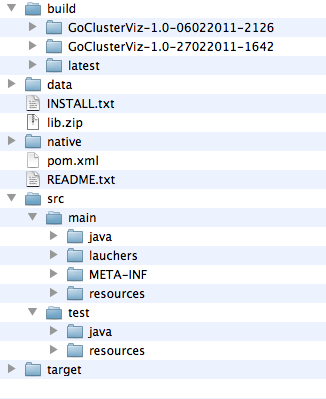
\includegraphics[scale=0.6]{pictures/thesis_folder_structure.png}
\caption{Thesis folder structure}
\label{THESIS_FOLDER_STRUCTURE}
\end{figure}

Second necessary part of the normal development process is revision control. "Revision control, also known as version control or source control (and an aspect of software configuration management or SCM), is the management of changes to documents, programs, and other information stored as computer files. It is most commonly used in software development, where a team of people may change the same files. Changes are usually identified by a number or letter code, termed the "revision number", "revision level", or simply "revision". For example, an initial set of files is "revision 1". When the first change is made, the resulting set is "revision 2", and so on. Each revision is associated with a timestamp and the person making the change. Revisions can be compared, restored, and with some types of files, merged."~\cite{REVISION_CONTROL}


During thesis development was used Git version control system. "Git is a distributed revision control system with an emphasis on speed. Git was initially designed and developed by Linus Torvalds for Linux kernel development. Every Git working directory is a full-fledged repository with complete history and full revision tracking capabilities, not dependent on network access or a central server. Git's current software maintenance is overseen by Junio Hamano. Git is free software distributed under the terms of the GNU General Public License version 2. after he claimed that Andrew Tridgell had reverse-engineered the BitKeeper protocols.)
Torvalds wanted a distributed system that he could use like BitKeeper, but none of the available free systems met his needs, particularly his performance needs."~\cite{GIT} Git allows to store and work local on machine but for more safety reasons all source code stored on GitHub. GitHub is a web-based hosting service for software development projects that use the Git revision control system. GitHub provides free hosting open-source project. Thesis project home page on GitHub is \url{http://github.com/vadyalex/thesis} and source code url is \url{git://github.com/vadyalex/thesis.git}

\begin{figure}[h!]
\centering
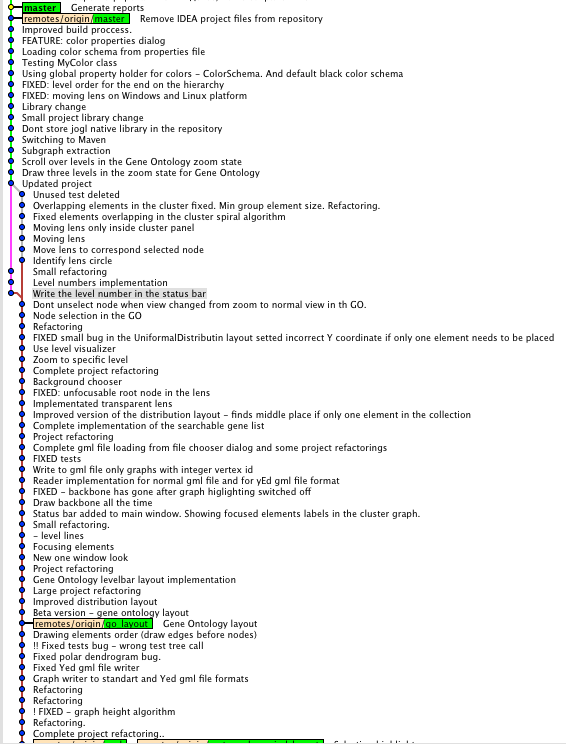
\includegraphics[scale=0.6]{pictures/commit_graph_gitk.png}
\caption{Commit graph of the local repository made by gitk tool}
\end{figure}


\subsection{Java Graph Libraries Overview}


There are overview of a few libraries for working with graphs in Java

\begin{enumerate}

\item
Java Graph Editing Framework (GEF)~\cite{GEF}

The aim of project consists in generation of library for graph editing, which can be used for construction of high-end (high-quality) custom applications for working with graphs.
GEF facilities (opportunities):
\begin{itemize}
	\item simple and clear design, which allows a developer to expand library's functionality
	\item Node-Port-Edge model of graph's presentation, which permits to perform overwhelming majority of tasks occurring in working with graphs applications
	\item future XML-based format support (SVG)
\end{itemize}

\item
ILOG JViews ~\cite{ILOG_Jview}

ILOG JViews gives (grants) components, aimed for using in custom applications, and also in common with Ajax and Eclipse platform.

\item
JGraphT~\cite{JGraphT}

JGraphT is open source library, which provides with mathematical tool of graphs theory. JGraphT supports different kinds of graphs, including: oriented and unoriented graphs, graphs with weighted/non weighted/nominate (named) or anything else arc format, appointed 	by user, non upgradeable graphs - supported access to internal graphs in "Read Only" mode. Listenable graphs: allows outer listener to trace events appearance; sub graphs: graphs which are a view about other graphs. Being a powerful feature, JGraphT has been 	developed as easy and type-safe (with Java code generators use) feature for working with 	graphs. For example, any object can be node of a graph. You can build graphics on basis of: line, URL, XML documents and so forth, you can even build graphs of graphs.

\item
Java Universal Network / Graph Framework (JUNG)~\cite{JUNG}

"JUNG � the Java Universal Network/Graph Framework--is a software library that provides a common and extendible language for the modeling, analysis, and visualization of data that can be represented as a graph or network. It is written in Java, which allows JUNG-based applications to make use of the extensive built-in capabilities of the Java API, as well as those of other existing third-party Java libraries.


The JUNG architecture is designed to support a variety of representations of entities and their relations, such as directed and undirected graphs, multi-modal graphs, graphs with parallel edges, and hypergraphs. It provides a mechanism for annotating graphs, entities, and relations with metadata. This facilitates the creation of analytic tools for complex data sets that can examine the relations between entities as well as the metadata attached to each entity and relation.
The current distribution of JUNG includes implementations of a number of algorithms from graph theory, data mining, and social network analysis, such as routines for clustering, decomposition, optimization, random graph generation, statistical analysis, and calculation of network distances, flows, and importance measures (centrality, PageRank, HITS, etc.).


JUNG also provides a visualization framework that makes it easy to construct tools for the interactive exploration of network data. Users can use one of the layout algorithms provided, or use the framework to create their own custom layouts. In addition, filtering mechanisms are provided which allow users to focus their attention, or their algorithms, on specific portions of the graph.


As an open-source library, JUNG provides a common framework for graph/network analysis and visualization. We hope that JUNG will make it easier for those who work with relational data to make use of one anothers' development efforts, and thus avoid continually re-inventing the wheel."~\cite{JUNG_OVERVIEW}


JUNG library is widely used in differ amount of projects. Here is a list of projects using JUNG:

\begin{itemize}

\item ExtC: an Eclipse plug-in that is useful for locating large, noncohesive classes and for recommending how to split them into smaller, more cohesive classes. (Keith Cassell)~\cite{EXTC}

\item Djinn: a tool for visualizing java artifacts dependencies in a project: jars, directories, packages, classes. (Fabien Benoit)~\cite{DJINN}

\item Angur: An XML visualization/WYSWYG Editor (Amir Mohammad shahi)~\cite{ANGUR}

\item RDF Gravity: a tool for visualizing RDF/OWL graphs/ontologies. (Sunil Goyal, Rupert Westenthaler)~\cite{RDF_GRAVITY}

\item GUESS from HP Labs is a database-driven network analysis tool that provides flexible visualizations, scripting capabilities with Python/Jython, and interfaces with JUNG to let users take advantage of its algorithm library. (Eytan Adar, David Feinberg)~\cite{GUESS}

\item ADAPTNet is an applet that visualises the families of short oligo microarray probesets associated through common gene transcripts. (Michal Okoniewski, Tim Yates)~\cite{ADAPTNET}

\item Augur~\cite{AUGUR} is a visualization tool designed to support the distributed software development process. (Jon Froehlich)~\cite{AUGUR_2}

\item Ariadne is an Eclipse plug-in (under development) that links technical and social dependencies. (Cleidson de Souza et al.)~\cite{ARIADNE}

\item Netsight is a proof-of-concept tool for the visual exploratory data analysis of large-scale network and relational data sets. (Yan-Biao Boey, Joshua O'Madadhain, Scott White, Padhraic Smyth)~\cite{NETSIGHT}

\item InfoVis CyberInfrastructure provides an unified architecture in which diverse data analysis, modeling and visualization algorithms can be plugged in and run.~\cite{INFOVIS_CYBERINFRASTRUCTURE}

\item PWComp is a graph comparative metabolic pathway tool. (Joshua Adelman, Josh England, Alex Chen)~\cite{PWCOMP}

\item Google Cartography, featured in Google Hacks, uses the Google Search API to build a visual representation of the interconnectivity of streets in an area. (Richard Jones)~\cite{GOOGLE_CARTOGRAPHY}

\item GINY is a project with similar aims to that of JUNG, which contains some code derived from JUNG. (Rowan Christmas)~\cite{GINY}

\item GraphExplore is a JAVA application that renders networks of objects in a graphical form, which uses modified forms of the JUNG layout algorithm implementations. (Quanli Wang)~\cite{GRAPHEXPLORER}

\item TOTEM (TOolbox for Traffic Engineering Methods) provides a framework where researchers can integrate their traffic engineering algorithms. These algorithms can therefore be applied on models of real networks. The TOTEM toolbox also gives network operators the opportunity to experiment the currently developed traffic engineering algorithms on their own network. Today, the TOTEM toolbox already federates a large set of traffic engineering algorithms published in the scientific literature. This project uses JUNG for the graphical representation of the network topology. (S. Balon, O. Delcourt, J. Lepropre and F. Skivee)~\cite{TOTEM}

\item D2K ("Data to Knowledge") is a visual programming environment for building complicated data mining applications; T2K is a library of D2K modules that implements sophisticated algorithms for text analysis. Each of these uses JUNG for network visualization.~\cite{D2K}

\item graphBuilder is an application that allows users to build network representations of relational databases and data files. It has been designed as a tool for exploring online scientific data repositories. (Ben Raymond)~\cite{GRAPHBUILDER}

\item Semiophore is an application for exploring large graphs where there are many variables on both nodes and links (including time-based/event variables). It works with a relationnal database. It provides several visualization approaches. One of them is based on JUNG. It provides several analysis routines, featuring SNA measures among them. User can interact with the network : dynamic multi-variables filtering, dynamic aggregation, network editing and production of quicktime videos from longitudinal analysis are possible. Semiophore can handle text/XML documents with NLP information extraction and text summarization routines [English and French support only] in order to automatically build network maps of actors/information.~\cite{SEMIOPHORE}

\item Xholon uses JUNG to represent and visualize networks such as biochemical pathways and models (screenshots). (Ken Webb)~\cite{XHOLON}

\item Flink is a website presenting the social networks and research activity of Semantic Web researchers based on a number of sources (web pages, publication databases, email archives, FOAF data). Flink uses JUNG for network representation and visualization as well as for computing network measures. Flink has won 1st prize at the Semantic Web Challenge~\cite{SWC} of 2004. (Peter Mika)~\cite{FLINK}

\item T-Prox(approve sites) is a proxy, designed to be used for usability analyzes of websites. It uses JUNG to visualize the users path through the site. (Sven Lilienthal)~\cite{T_PROX}

\item Simple C-K Editor is a visualisation tool built on the C-K Design Theory. Its main purpose is to provide an easy tool to create, manipulate, edit and print C-K diagrams.~\cite{SIMPLE_C_K_EDITOR}

\item PCOPGene is web-based application to analise microarray data with large sample-series. The user can identify several kinds of non-linear expression relationships inside the gene network, study the expression dependence fluctuations in detail, and crossing the results with external biomedical data-servers.~\cite{PCOPGENE}

\end{itemize}

\end{enumerate}

There are a lot more graph visualization frameworks for Java: Piccolo~\cite{Piccolo}, The Visualization Toolkit (VTK)~\cite{VTK}, The InfoVis Toolkit~\cite{InfoVis_Toolkit}, Improvise~\cite{Improvise}. All of them can be used as for storing and visualizing graphs and networks.


In the scope of current thesis work was used JUNG graph library to store graph structures.

\subsection{OpenGL visualization standart}
\label{opengl}
"OpenGL is a software interface to graphics hardware. This interface consists of about 120 distinct commands, which you use to specify the objects and operations needed to produce interactive three-dimensional applications.


OpenGL is designed to work efficiently even if the computer that displays the graphics you create isn't the computer that runs your graphics program. This might be the case if you work in a networked computer environment where many computers are connected to one another by wires capable of carrying digital data. In this situation, the computer on which your program runs and issues OpenGL drawing commands is called the client, and the computer that receives those commands and performs the drawing is called the server. The format for transmitting OpenGL commands (called the protocol) from the client to the server is always the same, so OpenGL programs can work across a network even if the client and server are different kinds of computers. If an OpenGL program isn't running across a network, then there's only one computer, and it is both the client and the server.


OpenGL is designed as a streamlined, hardware-independent interface to be implemented on many different hardware platforms. To achieve these qualities, no commands for performing windowing tasks or obtaining user input are included in OpenGL; instead, you must work through whatever windowing system controls the particular hardware you're using. Similarly, OpenGL doesn't provide high-level commands for describing models of three-dimensional objects. Such commands might allow you to specify relatively complicated shapes such as automobiles, parts of the body, airplanes, or molecules. With OpenGL, you must build up your desired model from a small set of geometric primitive - points, lines, and polygons."~\cite{THE_RED_BOOK}


There are many wrappers over OpenGL for developing on different programming languages. One of the favourite are JOGL and LWJGL.


"The Lightweight Java Game Library (LWJGL) is a solution aimed directly at professional and amateur Java programmers alike to enable commercial quality games to be written in Java. LWJGL provides developers access to high performance crossplatform libraries such as OpenGL (Open Graphics Library) and OpenAL (Open Audio Library) allowing for state of the art 3D games and 3D sound. Additionally LWJGL provides access to controllers such as Gamepads, Steering wheel and Joysticks. All in a simple and straight forward API.


LWJGL is not meant to make writing games particularly easy; it is primarily an enabling technology which allows developers to get at resources that are simply otherwise unavailable or poorly implemented on the existing Java platform. We anticipate that the LWJGL will, through evolution and extension, become the foundation for more complete game libraries and "game engines" as they have popularly become known, and hide some of the new evils we have had to expose in the APIs.


LWJGL is available under a BSD license, which means it's open source and freely available at no charge."~\cite{LWJGL}


In the thesis used JOGL wrapper library over OpenGL. "Java OpenGL (JOGL) is a wrapper library that allows OpenGL to be used in the Java programming language. It was originally developed by Kenneth Bradley Russell and Christopher John Kline, and was further developed by the Sun Microsystems Game Technology Group. As of 2010, it is an independent open source project under a BSD license. It is the reference implementation for Java Bindings for OpenGL (JSR-231).


The base OpenGL C API and associated operation system API, are accessed in JOGL via Java Native Interface (JNI) calls. As such, the underlying system must support OpenGL for JOGL to work. JOGL differs from some other Java OpenGL wrapper libraries in that it merely exposes the procedural OpenGL API via methods on a few classes, rather than trying to map OpenGL functionality onto the object-oriented programming paradigm. Indeed, most of the JOGL code is autogenerated from the OpenGL C header files via a conversion tool named GlueGen, which was programmed specifically to facilitate the creation of JOGL.


This design decision has both its advantages and disadvantages. The procedural and state machine nature of OpenGL is inconsistent with the typical method of programming under Java, which is bothersome to many programmers. However, the straightforward mapping of the OpenGL C API to Java methods makes conversion of existing C applications and example code much simpler. The thin layer of abstraction provided by JOGL makes runtime execution quite efficient, but accordingly is more difficult to code compared to higher-level abstraction libraries like Java3D. Because most of the code is autogenerated, changes to OpenGL can be rapidly added to JOGL."~\cite{JOGL}


\subsection{IO layer Implementation}

\subsection{Gene Ontology Visualization Implementation}
\subsection{Cluster Visualization Implementation}